\documentclass[12pt]{article}

\usepackage[utf8]{inputenc}
\usepackage[T1]{fontenc}
\usepackage{mathptmx}
\usepackage[brazil]{babel}
\usepackage[a4paper,margin=2.5cm]{geometry}
\usepackage{graphicx}
\usepackage{amsmath}
\usepackage{amssymb}
\usepackage{float}
\usepackage{booktabs}
\usepackage{indentfirst}
\usepackage{hyperref}

\setlength{\parindent}{1.25cm}
\setlength{\parskip}{0.5em}

\begin{document}

% ======================================================================
% Capa
% ======================================================================
\begin{titlepage}
    \centering
    \vspace*{1cm}

    \vspace{1.5cm}

    {\large Universidade de São Paulo}\\[0.2cm]
    {\large Instituto de Ciências Matemáticas e de Computação}\\[1.5cm]

    {\large SCC0252 -- Visualização Computacional}\\[0.2cm]
    {\large Prof. Jean R. Ponciano}\\[2.5cm]

    {\LARGE \textbf{Análise e comparação de cursos do ICMC a partir de gráficos}}\\[3cm]

    {\large
    Gabriel Martins Monteiro -- N\textsuperscript{o} USP: 14572099\\[0.3cm]
    Hélio Márcio Cabral Santos -- N\textsuperscript{o} USP: 14577862\\[0.3cm]
    Eduardo Pereira de Luna Freire -- N\textsuperscript{o} USP: 14567304\par}
\end{titlepage}

% ======================================================================
% Corpo do relatório
% ======================================================================

\section{Apresentação}

O projeto visa comparar os diferentes cursos do ICMC por meio de gráficos,
buscando evidenciar semelhanças e diferenças na estrutura curricular que não
são facilmente percebidas por meio de tabelas.

O problema surgiu da necessidade de conseguir comparar os cursos de forma
rápida e visual. Por exemplo, muitos alunos possuem dúvida ao escolher o curso
de ingresso no ICMC, perguntando qual a diferença entre eles etc. O projeto,
por meio dos gráficos, visa ilustrar essa diferença de forma visual, mostrando
como os cursos diferem em carga horária, distribuição de disciplinas entre
departamentos, créditos-aula/trabalho, entre outros.

\section{Introdução}

O conjunto de dados utilizado é composto pela grade curricular de cinco cursos
do ICMC: Ciências da Computação, Sistemas de Informação, Ciência de Dados,
Estatística e Matemática Aplicada.

Da página do Júpiter Web, extraíram-se as disciplinas por semestre, com uma
tabela para cada semestre de cada curso organizada em pastas; cada tabela
contém o departamento, o crédito-aula e o crédito-trabalho, a carga horária,
extensão e nome de cada disciplina.

O conjunto é formado por tabelas semestrais, com variáveis textuais para nomes
e departamentos e variáveis numéricas para créditos, carga horária e extensão.
O tamanho do conjunto corresponde ao número de disciplinas semestrais dos cinco
cursos.

A partir de uma análise preliminar do conjunto de dados, foram levantadas
quatro questões que podem ser respondidas ou exploradas. A primeira questiona
como os diversos cursos evoluem sua carga horária ao longo dos semestres, isto
é, se todos evoluem da mesma forma ou se alguns diminuem a carga horária de
forma mais rápida. A segunda questiona como as disciplinas de cada departamento
estão distribuídas em cada curso, por exemplo, se o curso de computação tem
mais disciplinas de matemática dos departamentos SMA e SME do que o curso de
Sistemas de Informação. A terceira questiona como se comparam os créditos em
cada curso, verificando se alguns cursos possuem mais crédito-trabalho em
percentual do que outros. A quarta questiona como se comporta a dispersão de
carga horária das matérias nos cursos escolhidos.

\section{Pré-processamento}

As páginas do Júpiter Web que mostram a grade curricular de cada curso estão em
formato não estruturado, o que exigiu uma etapa de pré-processamento. Ao
analisar o HTML da página de grade curricular do Júpiter Web, notou-se que os
dados estavam organizados em tags de tabela, o que facilitou o trabalho, pois
seria possível converter essa tabela para um arquivo CSV.

O processo adotado iniciou-se com o download das páginas HTML de cada um dos
cinco cursos extraídos. Em seguida, utilizou-se um script em Python que
convertia a tabela HTML para um CSV.

Após a conversão, realizou-se o pré-processamento do CSV para remover conteúdo
inútil, incluindo códigos de JavaScript incorporados à tabela. O CSV gerado foi
então dividido em várias tabelas, uma para cada semestre do curso.

Dentro de cada tabela, os dados foram limpos e transformados, como no caso da
limpeza do código da disciplina para deixar somente o departamento.

Para realizar essa tarefa, utilizou-se um script em Python que convertia a
página HTML em uma tabela CSV e uma combinação de scripts shell em Linux com
ferramentas como sed, que manipula expressões regulares, e grep, que filtra
dados.

Algumas matérias não eram de departamentos do ICMC e, por isso, estão com
departamento vazio na base de dados. O departamento vazio será interpretado
como matéria multidisciplinar, pois envolve outros departamentos.

\section{Análise Visual}

\subsection{Evolução da Carga Horária de Cada Curso por Semestre}

\begin{figure}[H]
    \centering
    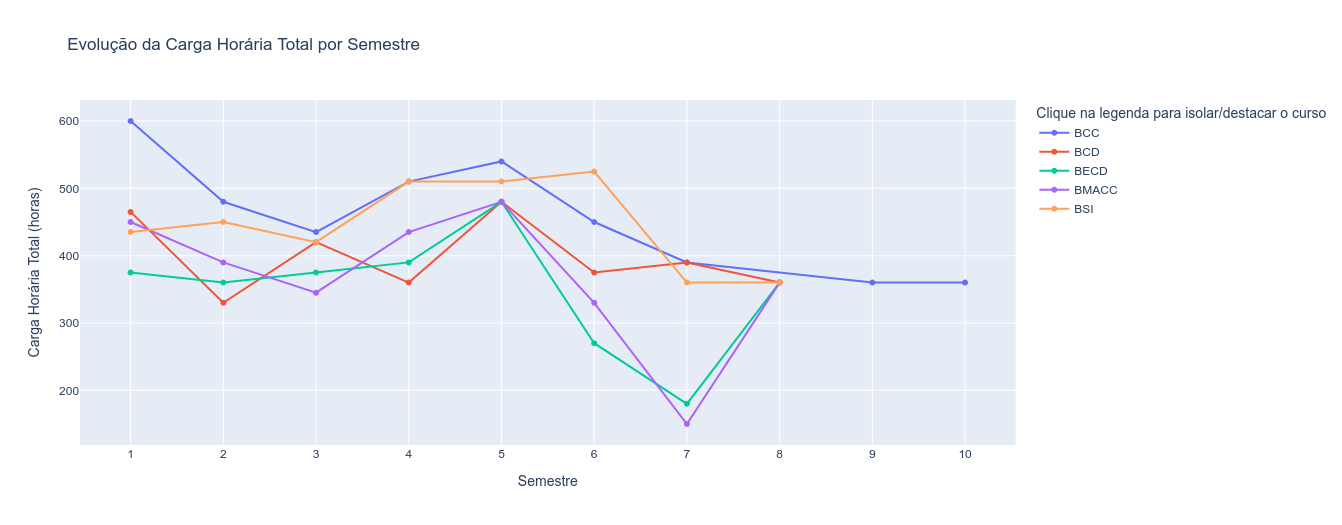
\includegraphics[width=\textwidth]{graficos/ch-total.png}
    \caption{Evolução da carga horária de cada curso por semestre.}
    \label{fig:ch-total}
\end{figure}

Para a análise da evolução da carga horária de cada curso ao longo dos
semestres, foi escolhido o gráfico de linhas, apresentado na
Figura~\ref{fig:ch-total}. Esse tipo de gráfico favorece a comparação da
evolução dos cursos entre si, pois permite observar tendências gerais, como a
redução da carga horária em todos os cursos ou o crescimento abrupto de algum
curso em determinado semestre.

Além disso, o gráfico permite interatividade, de modo que o leitor pode
escolher quais linhas de quais cursos devem permanecer visíveis. Com isso,
torna-se possível comparar dois cursos específicos ou acompanhar a evolução de
um único curso com maior clareza.

\subsection{Comparação da Distribuição de Carga Horária por Departamento}

\begin{figure}[H]
    \centering
    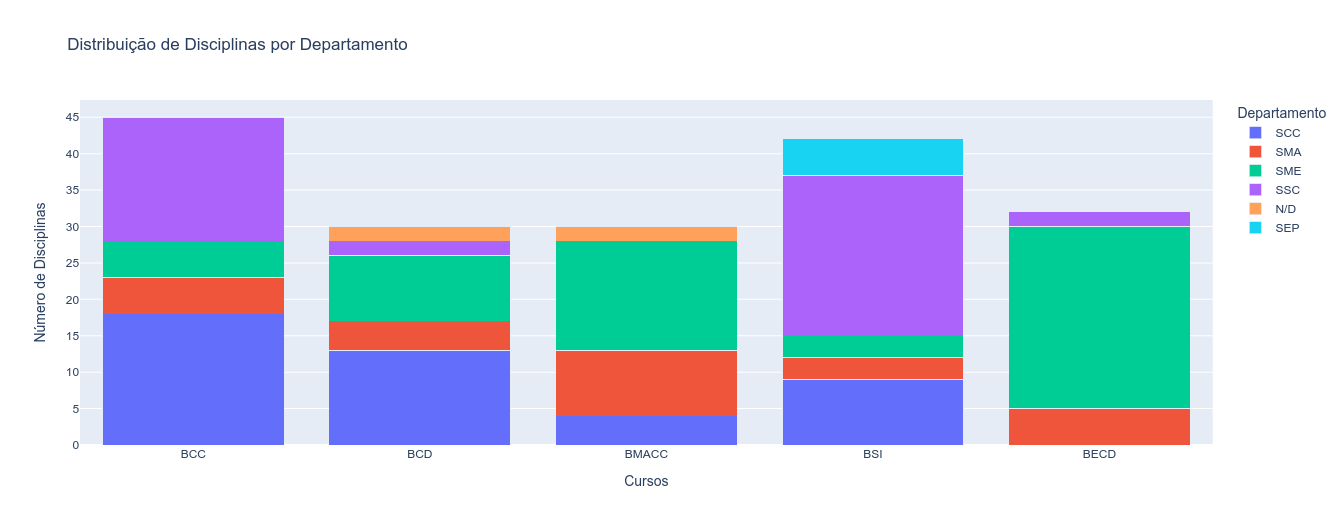
\includegraphics[width=\textwidth]{graficos/dist-disciplinas.png}
    \caption{Comparação da distribuição de carga horária por departamento.}
    \label{fig:dist-disciplinas}
\end{figure}

Para a comparação da distribuição de carga horária por departamento, foi
utilizado um gráfico de barras empilhadas, mostrado na
Figura~\ref{fig:dist-disciplinas}. Esse tipo de gráfico é adequado para
analisar a composição do todo, isto é, as partes em relação ao todo, e para
entender como as subcategorias contribuem para o valor total.

Dessa forma, o leitor pode identificar rapidamente quais cursos apresentam
maior porcentagem de carga horária relacionada a determinada área, como
computação ou matemática. A vantagem desse tipo de representação é que ele
enfatiza a comparação entre o total e as proporções de cada subcategoria.

Além disso, o gráfico permite que o leitor passe o mouse sobre os elementos e
verifique os valores específicos dos dados, como forma de interatividade.

\subsection{Comparação entre Créditos-Aula e Créditos-Trabalho por Curso}

\begin{figure}[H]
    \centering
    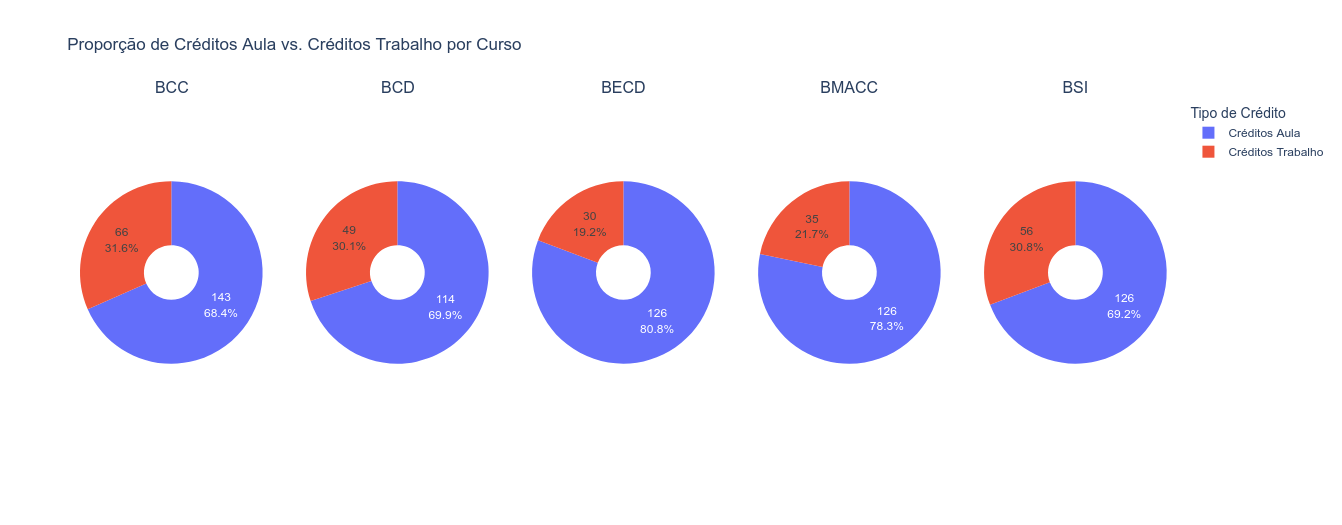
\includegraphics[width=\textwidth]{graficos/cred.png}
    \caption{Comparação entre créditos-aula e créditos-trabalho por curso.}
    \label{fig:cred}
\end{figure}

Para a comparação entre créditos-aula e créditos-trabalho por curso, foram
utilizados gráficos de pizza, apresentados na Figura~\ref{fig:cred}. Como há
apenas dois dados sendo comparados, o gráfico de pizza representa de forma
visual e concreta a porcentagem de maneira equivalente para todos os cursos,
que é justamente o objetivo da análise.

Nesse caso, não se busca comparar o tamanho do todo, mas apenas as proporções
entre créditos-aula e créditos-trabalho. Assim, há um gráfico de pizza para
cada curso, permitindo que o leitor rapidamente verifique qual curso possui
maior crédito-trabalho proporcionalmente.

O gráfico também permite interatividade para que o leitor veja o valor exato de
cada parcela.

\subsection{Distribuição de Carga Horária Individual das Disciplinas por Curso}

\begin{figure}[H]
    \centering
    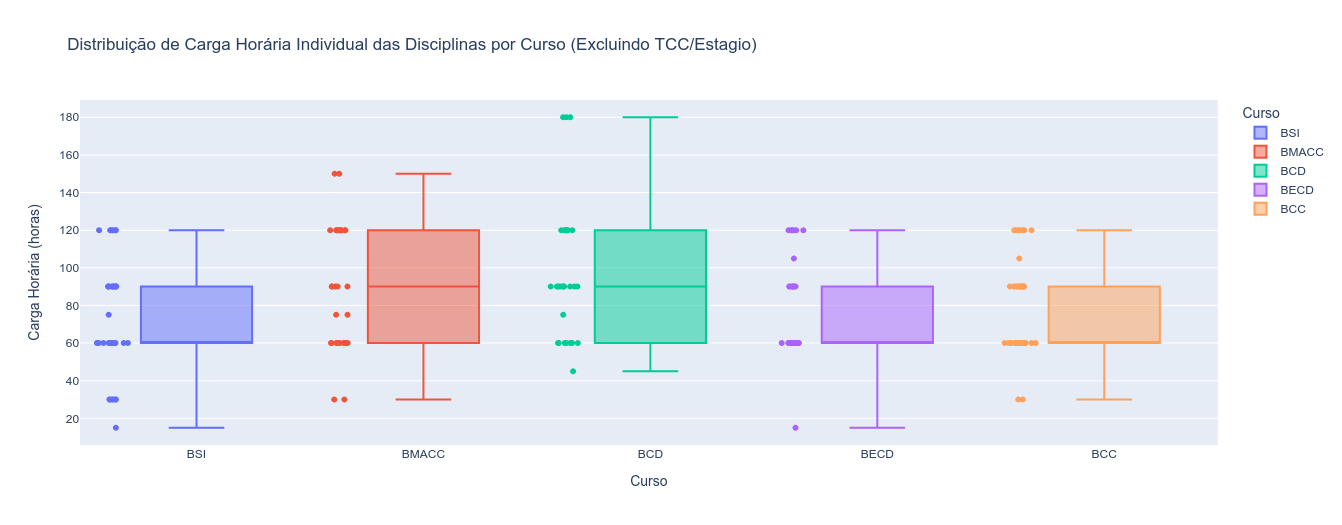
\includegraphics[width=\textwidth]{graficos/ch-ind.png}
    \caption{Distribuição de carga horária individual das disciplinas por curso.}
    \label{fig:ch-ind}
\end{figure}

Para a comparação da distribuição de carga horária individual das disciplinas
por curso, foram utilizados boxplots, apresentados na Figura~\ref{fig:ch-ind}.
Esse tipo de gráfico permite que o leitor identifique rapidamente a mediana, a
região de concentração dos dados e a presença de outliers.

Também possibilita comparar as distribuições entre os cursos, como a mediana e
o valor máximo de cada um. O gráfico permite interatividade para que o leitor
possa consultar os valores exatos de mediana, quartis e demais informações da
distribuição.

\section{Discussões Preliminares}

% Esqueleto vazio: inserir aqui os insights obtidos, a interpretação crítica dos resultados, as limitações e a reflexão sobre o processo e lições aprendidas.

\section{Próximos Passos}

% Esqueleto vazio: inserir aqui as direções para a segunda etapa do projeto, com novas questões a serem exploradas ou o aprofundamento de alguma questão específica.

\end{document}
